\documentclass[11pt,fleqn,a4paper,]{LegrandOrangeBook}
\addbibresource{sample.bib} % Bibliography file
\definecolor{ocre}{RGB}{243, 102, 25} 
\chapterimage{orange1.jpg} 
\chapterspaceabove{6.5cm}
\chapterspacebelow{6.75cm} 

%----------------------------------------------------------------------------------------
\begin{document}
\section{Ley de Coulomb}
La ley de Coulomb establece de la fuerza \textit{F} entre dos cargas \textit{$Q_1$} y \textit{$Q_2$} son:
\begin{itemize}
\item A lo largo de la linea que los une.
\item Directamemte proporcional al producto \textit{$Q_1Q_2$} de las cargas.
\item Inversamente proporcional a la distancia \textit{R} que los separa
\end{itemize}
\begin{theorem}[Ley de Coulomb]
\begin{equation}
\label{eq:eqCoulomb}
F=\frac{kQ_1Q_2}{R^2}
\end{equation}
Donde:\\
\begin{itemize}
\item \textit{Q}: Cargas en Coulombs(C).
\item R: Distancia en metros(m).
\item F: Fuerza Newtons(N).
\end{itemize}
Constantes:
\begin{align*}
&\epsilon_0=8.854 \times 10^{-12}\simeq \frac{10^{-9}}{36\pi}F/m
&k=\frac{1}{4\pi\epsilon_0}\simeq 9\times 10^9 m/F
\end{align*}
\end{theorem}
Si las cargas $\textit{Q}_1$ y $\textit{Q}_2$ están localizadas en puntos cuyas posiciones están de forma vectorial $\textit{r}_1$ y $\textit{r}_2$(figura ), así la fuerza de $\textbf{F}_{12}$\footnote{Se lee: La fuerza de la carga 1 a la carga 2} sobre la carga 2 debido a la carga 1 esta dado por:
\begin{multicols}{2}
\begin{equation}
\boxed{F_{12}=\frac{Q_1Q_2}{4\pi\epsilon_0R^2}\textbf{a}_{R_{12}}}
\end{equation}
Sean n cargas y se desea hallar la fuerza resultante en una carga Q, se usa el \textit{principio de superposición}. Este principio establece: Si existen N cargas $Q_1, Q_2,...,Q_N$ y seas sus vectores posición $r_1, r_2,.., r_N$ la fuerza resultante en la carga Q es la sumatoria de las fuerzas de cada una de las cargas:
\begin{displaymath}
F_Q=F_1+F_2+F_3+\ldots +F_N
\end{displaymath}
o:
\begin{equation}
\boxed{F=\frac{Q}{4\pi\epsilon_0}\sum^N_{k=1}\frac{Q_k(r-r_k)}{|r-r_k|^3}}
\end{equation}
\columnbreak
  \begin{center}
    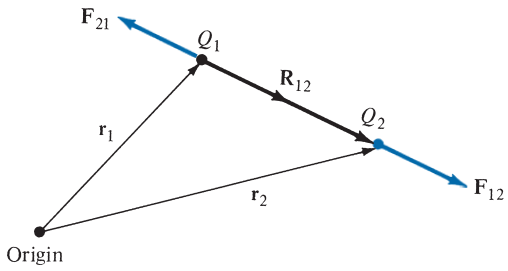
\includegraphics[scale=0.4]{CamposMag/CM10.png}
  \end{center}
\end{multicols}
\section{Intensidad de campo eléctrico}
La intensidad de campo eléctrico E es la fuerza que una unidad de carga positiva experimenta cuando se coloca en un campo eléctrico.
\begin{theorem}[Intensidad de campo eléctrico]
\begin{equation}
\label{eq:Intensidadcampoelectrico}
E=\frac{F}{Q}
\end{equation}
Donde:
\begin{itemize}
\item E: Intensidad de campo eléctrico(N/C) o Volts por metro(V/m).
\item F: Fuerza(N)
\item Q: Carga(Coulombs).
\end{itemize}
\end{theorem}
Para Q>0, el E esta en la misma dirección de la fuerza F. La intensidad de campo eléctrico en el punto \textbf{r} debido a una carga localizada en \textbf{r'} es obtenido:
\begin{equation}
E=\frac{Q(r-r')}{4\pi\epsilon_0|r-r'|^3}=\frac{Q}{4\pi\epsilon_0r^2}a_r
\end{equation}
Y bajo el mismo principio de superposición, la intensidad de campo eléctrico en el punto \textbf{r}:
\begin{equation}
\boxed{E=\frac{1}{4\pi\epsilon_0}\sum^N_{k=1}\frac{Q_k(r-r_k)}{|r-r_k|^3}}
\end{equation}
\section{Campo eléctrico creado por una distribución continua de carga en un punto}
Las cargas puntuales ocupan un muy pequeño espacio físico. Es posible tener distribuciones continuas: Es costumbre denotar la densidad de carga lineal $\rho_L$(C/m), la densidad de carga superficial $\rho_S$(C/$m^2$) y la carga volumétrica $\rho_V$(C/$m^3$).\footnote{No confundir este $\rho$ con subíndice con $\rho$ sin subíndice usado en coordenadas cilíndricas.}
\begin{align}
dQ=\rho_Ldl=\lambda dl &\rightarrow Q=\int_L\rho_Ldl\\
dQ=\rho_Sds=\sigma ds &\rightarrow Q=\int_S\rho_Sds\\
dQ=\rho_vdv=\rho dv &\rightarrow Q=\int_v\rho_vdv
\end{align}
El campo eléctrico debido a cada distribución de carga puede ser tomado como una sumatoria de los campos contribuidos por numerosas cargas:
\begin{align}
\vec{E}&=\int_Lk\lambda\frac{dl}{r^2}\vec{u}_r\\
\vec{E}&=\int_Sk\sigma\frac{ds}{r^2}\vec{u}_r\\
\vec{E}&=\int_Vk\rho\frac{dv}{r^2}\vec{u}_r
\end{align}
\section{Densidad de campo eléctrico}
\begin{definition}[Flujo Eléctrico]
Se dice que la \textbf{densidad de flujo eléctrico} es el número de líneas de fuerza por metro cuadrado de superficie, para una esfera de radio \textit{r}, esta dada por:
\begin{equation}
\vec{D}=\frac{q}{4\pi r^2}\vec{r}
\end{equation}
Así para el espacio libre:
\begin{equation}
\vec{D}=\vec{E}\epsilon_0
\end{equation}
Donde:\\
\begin{itemize}
\item E: Campo eléctrico(N/C ó V/m).
\item D: Densidad de flujo eléctrico(C/$m^2$).
\end{itemize}
Se define \textbf{flujo eléctrico} en términos de la densidad de flujo eléctrico, es decir:
\begin{equation}
\Psi=\int_S\textbf{D}\cdot d\textbf{S}
\end{equation}
\end{definition}
%----------------------------------------------------------------------------------------


\end{document}
